\section{Modelos de Localización}

\subsection{Introducción}

Los problemas de Localización constituyen uno de los grupos de problemas de Investigación Operativa que más se han aplicado en
la práctica. La característica común a todos ellos es la necesidad de situar algún objeto o instalación de la mejor manera
posible. Si los lugares donde pueden estar situados estos objetos están restringidos a un conjunto discreto (generalmente
infinito) estaríamos dentro de la \textit{localización discreta}, que es la que se va a tratar aquí.

En muchos problemas se tienen los siguientes elementos básicos. Hay $m$ puntos de demanda de cierto servicio que hay que
cubrir, y $n$ posibles puntos donde situar una ``instalación'' o punto de servicio. El problema es decidir el número y la
localización de los puntos de servicio de forma que se optimice cierto objetivo, que suele depender de los costos de
instalación y de los costos del servicio. Según los objetivos que se consideren se tienen los siguientes problemas básicos
de localización

\begin{itemize}
    \item Problemas de Cubrimiento Total (Set Covering).
    \item Problemas de Cubrimiento Máximo.
    \item Problemas de Localización de Midianas.
    \item Problemas de Localización de Centros de Emergencia.
    \item Problemas de Localización con Costos Fijos.
    \item Problemas de Distritos.
\end{itemize}

\noindent Se van a describir los Problemas de Localización con Costos Fijos básicos.

\subsection{Problema de Localización con Costos Fijos}

Sea $M=\{1,\dots,m\}$ el conjunto de los puntos de demanda de cierto servicio y $N=\{1,\dots,n\}$ el conjunto de puntos donde
puede estar situada la instalación. En este tipo de modelos se supone que cada punto de demanda $i\in M$ tiene una demanda
$d_i$ de cierto servicio y que para $j\in N$ hay un coste fijo $f_j$ de apertura o mantenimiento de la instalación. Además,
se tiene un costo variable o unitario $c_{ij}$ asociado a servir una unidad de demanda al cliente $i$ desde la instalación
$j$. Si suponemos que las instalaciones pueden servir cualquier cantidad de demanda se tiene el Modelo de Localización sin
Capacidades, que se formula tal que

\begin{alignat}{3}
    \text{minimizar:}   & \sum_{j=1}^n(f_{j}x_{j} + \sum_{i=1}^m\sum_{j=1}^n c_{ij}z_{ij})  &                           \\
    \text{sujeto a:}    & \sum_{j=1}^nz_{ij}=d_i                                            & i=1,\dots,m               \\
                        & \sum_{i=1}^nz_{ij}\leq Mx_j                                       & j=1,\dots,n               \\
                        & z_{ij}\geq 0                                                      & i=1,\dots,m\; j=1,\dots,n \\
                        & x_{j}\in\{0,1\}                                                   & j=1,\dots,n
\end{alignat}

\noindent donde $x_j$ son las variables de localización binarias, corresponden a las decisiones de apertura o no de las
instalaciones y $z_{ij}$ indican las cantidades que se sirven desde cada instalación hasta cada cliente o punto de demanda.

\vspace*{2mm}

Haciendo el cambio de variable $y_{ij}=\frac{z_{ij}}{d_i}$ la variable $y_{ij}$ indica la fracción de la demanda del cliente
$i$ cubierta desde la instalación $j$ quedando un modelo más comunmente usado tal que

\begin{alignat}{3}
    \text{minimizar:}   & \sum_{j=1}^n(f_{j}x_{j} + \sum_{i=1}^m\sum_{j=1}^n c_{ij}y_{ij}d_i)   &                           \\
    \text{sujeto a:}    & \sum_{j=1}^ny_{ij}=1                                                  & i=1,\dots,m               \\
                        & \sum_{i=1}^ny_{ij}\leq mx_j                                           & j=1,\dots,n               \\
                        & 0\leq y_{ij}\leq 1                                                    & i=1,\dots,m\; j=1,\dots,n \\
                        & x_{j}\in\{0,1\}                                                       & j=1,\dots,n
\end{alignat}

\noindent donde ahora ya no es preciso un $M$ lo suficientemente grande sino que vale con $m$ el número de puntos demanda. 

\vspace*{2mm}

Si para cada posible instalación $j\in N$ hay una capacidad $u_j$ para la demanda total que puede servir, se tiene el modelo 
de Localización con Capacidades siguiente

\begin{alignat}{3}
    \text{minimizar:}   & \sum_{j=1}^n(f_{j}x_{j} + \sum_{i=1}^m\sum_{j=1}^n c_{ij}y_{ij}d_i)   &                           \\
    \text{sujeto a:}    & \sum_{j=1}^ny_{ij}=1                                                  & i=1,\dots,m               \\
                        & \sum_{i=1}^nd_iy_{ij}\leq u_jx_j                                      & j=1,\dots,n               \\
                        & 0\leq y_{ij}\leq 1                                                    & i=1,\dots,m\; j=1,\dots,n \\
                        & x_{j}\in\{0,1\}                                                       & j=1,\dots,n
\end{alignat}

\noindent conocida como formulación débil. Añadiendo la restricción $y_{ij}\leq x_j$ para $j=1,\dots,n$ se refuerza
considerablemente la relajación lineal del problema, conocida como formulación fuerte.

En una variante de estos modelos se exige que cada punto de demanda será cubierto por una única instalación. Esta restricción
se conoce como de fuente única. En el caso del modelo sin capacidades la solución óptima siempre puede tomarse verificando
esta condición, pues al no haber capacidades, cada punto de demanda será servido por la instalación abierta más cercana. 

\newpage

Sin embargo, en el caso capacitado lo anterior ya no puede garantizarse y se obtiene así el modelo conocido como Modelo de
Localización con Capacidades y Fuente Única (SSCFL) siguiente

\begin{alignat}{3}
    \text{minimizar:}   & \sum_{j=1}^n(f_{j}x_{j} + \sum_{i=1}^m\sum_{j=1}^n c_{ij}y_{ij}d_i)   &                           \\
    \text{sujeto a:}    & \sum_{j=1}^ny_{ij}=1                                                  & i=1,\dots,m               \\
                        & \sum_{i=1}^nd_iy_{ij}\leq u_jx_j                                      & j=1,\dots,n               \\
                        & y_{ij}\in\{0,1\}                                                      & i=1,\dots,m\; j=1,\dots,n \\
                        & x_{j}\in\{0,1\}                                                       & j=1,\dots,n
\end{alignat}

\noindent donde tanto $x_j$ como $y_{ij}$ son variables binarias. El modelo es considerablemente más dificil de resolver que
el CFL normal, y generalmente debe recurriste al uso de heurísticas para su resolución aproximada.

\subsection{Algoritmo greedy ADD para UFLP}

Al enfrentar la evolución del coste fijo, coste por unidad y el coste total contra el número de instalaciones se obtiene el
siguiente gráfico

\begin{center}
    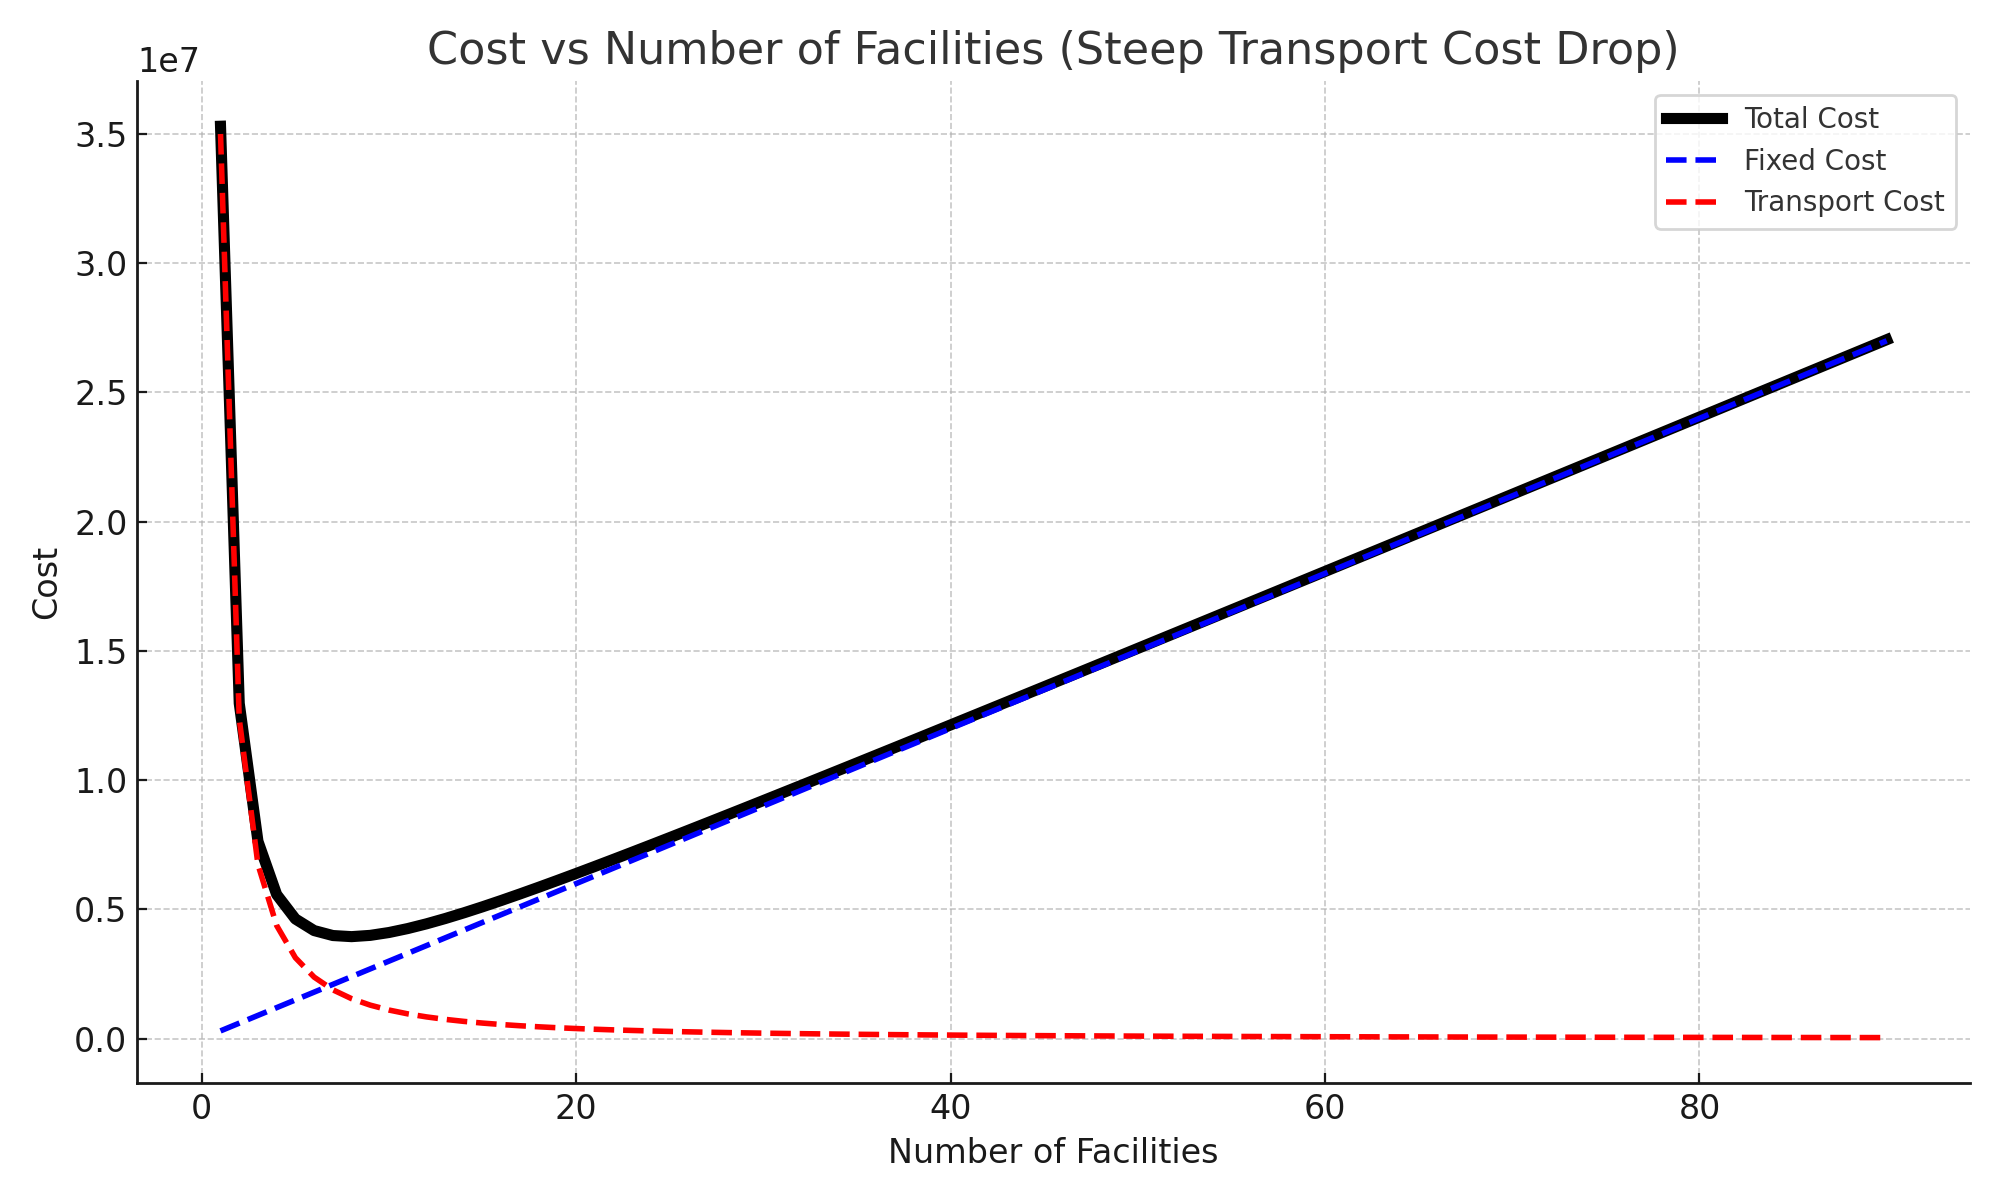
\includegraphics[width=0.8\textwidth]{img/GraficoCosteCentros.png}
\end{center}

\noindent se aprecia que existe un punto donde se minimiza el coste total justo donde se cruzan la función coste fijo y la
función coste por unidad. Esta propiedad la aprovechan los algoritmos greedy ADD y DROP para encontrar una solución factible
cercana al óptimo.

\vspace*{2mm}

Con el método ADD comenzamos en el lado izquierdo de la curva con una única instalación y se van añadiendo instalaciones de
dorma greedy mientras el costo total va disminuyendo (mayor decrecimiento y menor costo) y no se modifican elecciones hechas
hasta ese momento. Si no es posible mejorar añadiendo ninguna fabrica más hemos encontrado la solución.

Con el método DROP, se comienza en el lado derecho de la curva abriendo todas las intalaciones posibles y se van cerrando una
a una de forma greedy mientras el costo total disminuya.

Estos métodos fueron diseñados originalmente para el problema sin capacidades, y posteriormente se han extendido a muchos
otros problemas de localización. Para el problema UFLP se usan las siguientes notaciones. $z^h$ es el valor heurístico de la
solución actual y $S\subseteq N$ es el subconjunto de instalaciones abiertas. De forma equivalente, en lugar de $S$ puede
darse el array $x=(x_j)$ para $j=1,\dots,n$ donde $x_j=1$ si $j\in S$ y 0 en otro caso. Para el problema UFL es suficiente
representar la solución mediante el subconjunto $S\subseteq N$ o el array $x$, pues cada punto de demanda $i$ se asignará al 
punto de servicio abierto más cercano. Esto podemos darlo en otro array $y=(y_i)$ para $i=1,\dots,m$ con las asignaciones
actuales, es decir, $y_i$ es el punto de servicio abierto que sirve al punto de demanda $i$.

\subsection{Heurísticas de mejora para UFL}

Se parte de la solución factible obtenida con alguno de los procedimientos ADD o DROP de la sección anterior. Como a priori no
conocemos el número total de instalaciones o puntos de servicio que pueden ser abiertos en una solución óptima, los métodos de
mejora deben incluir la posibilidad de cerrar una instalación abierta (método drop), de abrir o añadir una nueva instalación
(método add), y también un posible intercambio (método swap), que consistiría en cerrar una y abrir otra simultaneamente.
Combinando estos métodos podemos generar entornos de solución sobre los que realizar busqueda local y aproximarnos a la
solución óptima.